\section{Homotopy approach to OCP}
\label{sec:Homotopy}  
%
Most of the time the minimum time optimal control problem cannot be solved directly because of the complexity and the lack of information of the system. In particular, the lagrange multiplier of the optimal control are undefined and initialised to zero.\\
A viable way to overcome this problematic is to use the continuation approach mentioned in the previous section. Therefore one can solve a simpler problem and step by step build the original OCP that want to solve.\\
This approach is particularly useful when dealing with closed circuit but can be used in general with open tracks.
%
\subsection{Cost function}
%
Lets suppose that the minimum time problem do not converge as it is for a track circuit. Another problem can be defined to be more complex in terms of cost function, but with a much simple solution.\\
Taking advantage of the previously defined additional terms of the cost function one can rewrite 
%
\begin{equation}
    \mathcal{J} = \int_{\zeta_L}^{\zeta_R} \frac{1}{\dot{s}} \mathrm{d}\zeta  
\end{equation}
%
In the full form
%
\begin{equation}
    \int_{\zeta_L}^{\zeta_R} \mathcal{L}(\zeta)\mathrm{d}\zeta = \mathcal{M}({\zeta_L},{\zeta_R}) + \int_{\zeta_L}^{\zeta_R} \mathcal{L}(\zeta) \mathrm{d}\zeta  
\end{equation}
%
with mayer term defined as 
%
\begin{equation}
    \begin{split}
    \mathcal{M}({\zeta_L},{\zeta_R}) = 
    &(\mathbf{x}(\zeta_L)-\mathbf{x_L})^T \mathbf{W_{L}} (\mathbf{x}(\zeta_L)-\mathbf{x_L}) + (\mathbf{x}(\zeta_R)-\mathbf{x_R})^T \mathbf{W_{R}} (\mathbf{x}(\zeta_R)-\mathbf{x_R}) + \dots\\
    &\dots + (\mathbf{x}(\zeta_L)-\mathbf{x}(\zeta_R))^T \mathbf{W_{LR}} (\mathbf{x}(\zeta_L)-\mathbf{x}(\zeta_R))
\end{split}
\end{equation}
%
and lagrange term
%
\begin{equation}
    \begin{split}
    \mathcal{L}({\zeta}) =  \int_{\zeta_L}^{\zeta_R} [ w_t + (\mathbf{x}(\zeta)-\mathbf{x_{ss}})^T \mathbf{W_{ss}}  (\mathbf{x}(\zeta)-\mathbf{x_{ss}}) ] \frac{1}{\dot{s}} \mathrm{d}\zeta
\end{split}
\end{equation}
%
\subsection{Solution approach}
%
The solution approach will follow some steps to converge to the desired problem. Lets recall that the key parameter here are the weights:
\begin{itemize}
    \item $w_t$
    \item $\mathbf{W_{ss}}$
    \item $\mathbf{W_{L}}$
    \item $\mathbf{W_{LR}}$
\end{itemize}
%
\subsection*{Problem 0}
%
The problem can be firstly solved by giving positive weight to the initial condition ($\mathbf{W_{L}}$) and the steady state ($\mathbf{W_{ss}}$), leaving the final condition free giving zero weight, zero also to the cyclic conditions ($\mathbf{W_{LR}}=\mathbf{0}$), and small or null to the minimum time effect $w_t=0$.\\
This yields a solution far from the minimum time desired. Generally speaking the trajectory will follow a minimum distance path along the track, if the $w_t$ is slightly different from zero. The states will start at the initial point and end in a different point with a certain state. This result can be seen in figure \ref{fig:Problem0}.\\
Summarising:
\begin{itemize}
    \item $w_t \ll 1 , \quad  w_t \in [0,10^{-2}] $
    \item $\mathbf{W_{ss}} \neq \mathbf{0} $
    \item $\mathbf{W_{L}} \neq \mathbf{0}  $
    \item $\mathbf{W_{LR}} = \mathbf{0}$
\end{itemize}
All matrices are diagonal and positive semi-definite since weights are non-negative and cross influence of states ais not considered. 
%
\begin{figure}[h!]
    \centering
    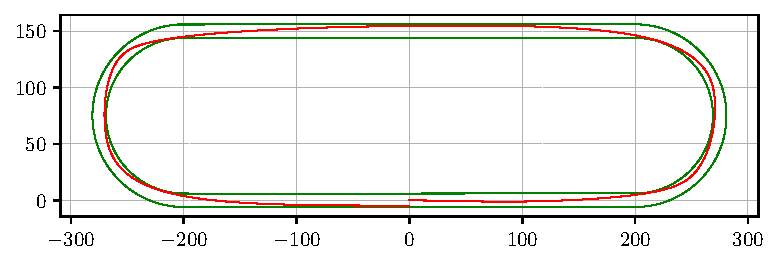
\includegraphics[width=\linewidth]{OCI/Track_Problem0.pdf}
    \caption{Trajectory solution of problem 0 in a simple circuit}
    \label{fig:Problem0}
\end{figure}
%
\subsection{Problem 1}
%
On the next step the weights are changed following this logic. The influence of the minimum time is pushed from the initial low value to 1. This will produce a behaviour that is in contrast with the steady state tracking. Therefore the weights of the steady state are pushed toward zero.\\
This is not done in one full step because in general the obtained solution are far different from the one obtained at Problem 0. Therefore, following the idea of small perturbation, the problem can be transformed in a series of fast converging problem that use as weights a linear interpolation. Lets consider $\nu$ an internal variable that can range in $[0,1]$ then we can summarize the problem 1 as 
\begin{itemize}
    \item $w_t = w_{t0} + (w_{t1}-w_{t0})\nu $
    \item $\mathbf{W_{ss}} = \mathbf{W_{ss0}} + (\mathbf{W_{ss1}}-\mathbf{W_{ss0}})\nu $
    \item $\mathbf{W_{L}} \neq \mathbf{0}  $
    \item $\mathbf{W_{LR}} = \mathbf{0}$
\end{itemize}
In this case $w_{t0}$ and $\mathbf{W_{ss0}}$ are the initial weights of the problem 0 while $w_{t1}$ and $\mathbf{W_{ss1}}$ are those wanted at the end of problem 1.\\
$s$ starts from a small value and gradually increase. At the end the problem 1 yield a solution that again is not a minimum lap time. In fact the initial condition are satisfied, the final condition are free and the lap is performed in the minimum time given the above mentioned constraints. It is important to highlight that up to this point the final and initial condition do not coincide as can be seen in figure \ref{fig:Problem1}
%
\begin{figure}[h!]
    \centering
    \includegraphics[width=\linewidth]{OCI/Track_Problem1.pdf}
    \caption{Trajectory solution of problem 1 in a simple circuit}
    \label{fig:Problem1}
\end{figure}
%
%
\subsection{Problem 2}
%
Following the same idea of the problem 1 one can use the solution obtained to guess a perturbed problem in which the weights of the cyclic condition are pushed from zero to the final value. Summarising the problem 2:
\begin{itemize}
    \item $w_t = 1 $
    \item $\mathbf{W_{ss}} = \mathbf{W_{ss1}} $
    \item $\mathbf{W_{L}} \neq \mathbf{0}  $
    \item $\mathbf{W_{LR}} = \mathbf{W_{LR0}} + (\mathbf{W_{LR2}}-\mathbf{W_{LR0}})\nu$
\end{itemize}
where $\mathbf{W_{ss1}}$ are the final weights of problem 1, $\mathbf{W_{LR0}}=0$ from previous problem and $\mathbf{W_{LR2}}$ are the final weights of the problem 2. Again the problem is transformed in a series of fast converging problems changing the cyclic weights wit a linear interpolation with the variable $\nu$.\\
The results will be a closed trajectory with initial and final condition that coincide. The lap is performed with the minimum time, but subjected to the imposed initial condition as can be seen in figure \ref{fig:Problem2}
%
\begin{figure}[h!]
    \centering
    \includegraphics[width=\linewidth]{OCI/Track_Problem2.pdf}
    \caption{Trajectory solution of problem 2 in a simple circuit}
    \label{fig:Problem2}
\end{figure}
%
\subsection{Problem 3}
%
In the last problem the idea is to free the initial condition. This can be done again with the continuation pushing toward zero the weight of the initial conditions $\mathbf{W_{L}}$. Summarizing the problem 3 we have
\begin{itemize}
    \item $w_t = 1 $
    \item $\mathbf{W_{ss}} = \mathbf{W_{ss1}} $
    \item $\mathbf{W_{L}}  = \mathbf{W_{L0}} + (\mathbf{W_{L3}}-\mathbf{W_{LR0}})\nu $
    \item $\mathbf{W_{LR}} = \mathbf{W_{LR2}}$
\end{itemize}
with $\mathbf{W_{L0}}$ the initial value of the initial conditions and $\mathbf{W_{L3}}$ the final.\\
The solution slowly shift from the fixed condition to a free one. This yield a trajectory that is closed, continuous and performed in the minimum time. This is in theory the perfect lap given the dynamic of the vehicle.(see figure \ref{fig:Problem3})
%
\begin{figure}[h!]
    \centering
    \includegraphics[width=\linewidth]{OCI/Track_Problem3.pdf}
    \caption{Trajectory solution of problem 3 in a simple circuit}
    \label{fig:Problem3}
\end{figure}
%
\subsection{Problem 4}
%
It is important to highlight that one can solve a further problem 4 to push tolerances of the boundaries. This is a slight variation and depend on how the constraints are formulated and regularised. Here in figure \ref{fig:Problem4} is reported the effect of pushing tolerances of the track bounds.
%
\begin{figure}[h!]
    \centering
    \includegraphics[width=\linewidth]{OCI/Track_Problem4.pdf}
    \caption{Trajectory solution of problem 4 in a simple circuit}
    \label{fig:Problem4}
\end{figure}
%
\subsection{Compare the problems}
%
In this section the results are collected in a single figure tu clearly observe the differences in the trajectories of the problem. (figure \ref{fig:ProblemCompare})
%
\begin{figure}[h!]
    \centering
    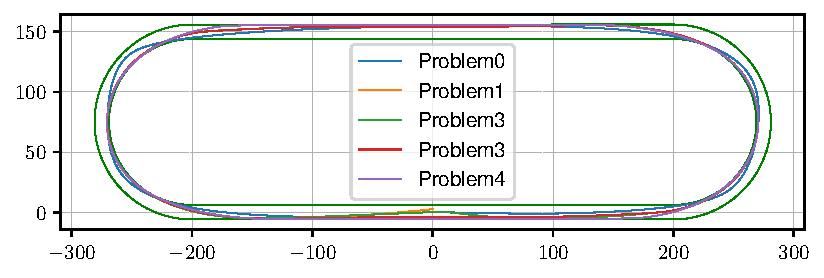
\includegraphics[angle=90,origin=c,height=0.9\linewidth]{OCI/Track_problemCompare.pdf}
    \caption{Trajectory comparison of the sequence of problems in a simple circuit}
    \label{fig:ProblemCompare}
\end{figure}
%